\ylDisplay{Läätse fookus} % Ülesande nimi
{Tundmatu autor} % Autor
{piirkonnavoor} % Voor
{2016} % Aasta
{P 8} % Ülesande nr.
{3} % Raskustase
{
% Teema: Valgusõpetus
\ifStatement
Joonisel on näidatud punkt $A$, kus laserkiir lõikab pärast läätsede läbimist optilist peatelge. Konstrueerige nõgusläätse fookuse $F_n$ asukoht. Lahendage ülesanne lisalehel.
\begin{center}
	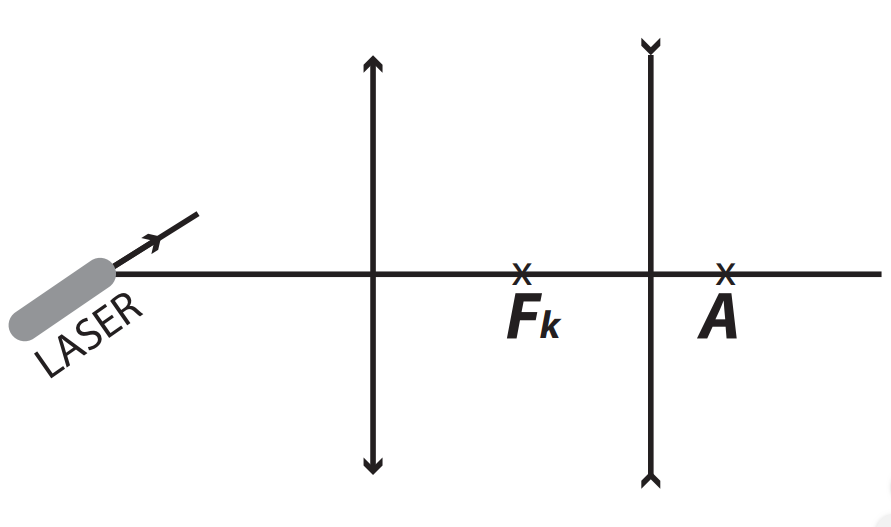
\includegraphics[width=0.5\linewidth]{2016-v2p-08-yl.PNG}
\end{center}
\fi


\ifHint
Ülesande lahendamisel on vaja konstrueerida laserkiire liikumine läbi läätsede, kasutades selleks abisirgeid, mis on paralleelsed laserkiirega ning läbivad läätsede keskpunkte.
\fi


\ifSolution
\begin{center}
	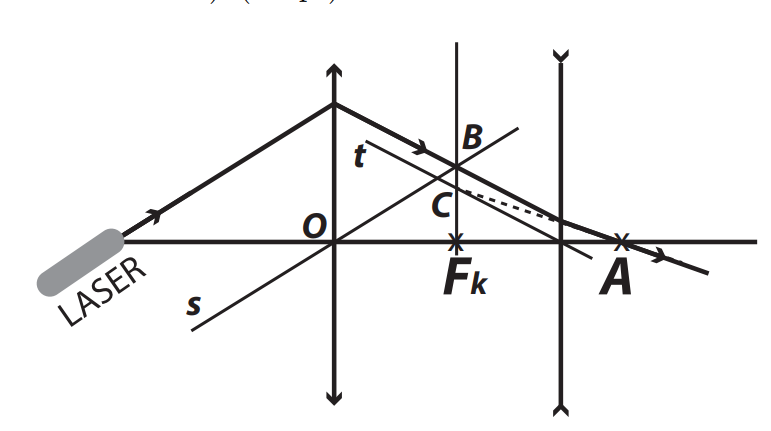
\includegraphics[width=0.5\linewidth]{2016-v2p-08-lah.PNG}
\end{center}
Joonistame laseri kiirega paralleelse optilise kõrvaltelje $s$. Kumerläätsele langenud optilise kõrvalteljega paralleelne kiir lõikab pärast murdumist läätses fokaaltasandit punktis $B$, kus lõikuvad optiline kõrvaltelg $s$ ja läätse fokaaltasand. (Fokaaltasand on tasand, mis on risti läätse optilise peateljega ja läbib fookust.) Et konstureerida valguskiire käik nõgusläätses, joonistame nõgusläätsele langevale kiirele paralleelse optilise kõrvaltelje $t$. Nõgusläätsele langenud optilise kõrvalteljega paralleelne kiir hajub pärast murdumist läätses, läbides punkti $A$, nii et hajunud kiire pikendus lõikab optilist kõrvaltelge punktis $C$, kus lõikuvad optiline kõrvaltelg ja fokaaltasand. Jooniselt on näha, et läätsede fokaaltasandid ühtivad, järelikult ühtivad ka nende fookused.
\fi
}
